\begin{center}
	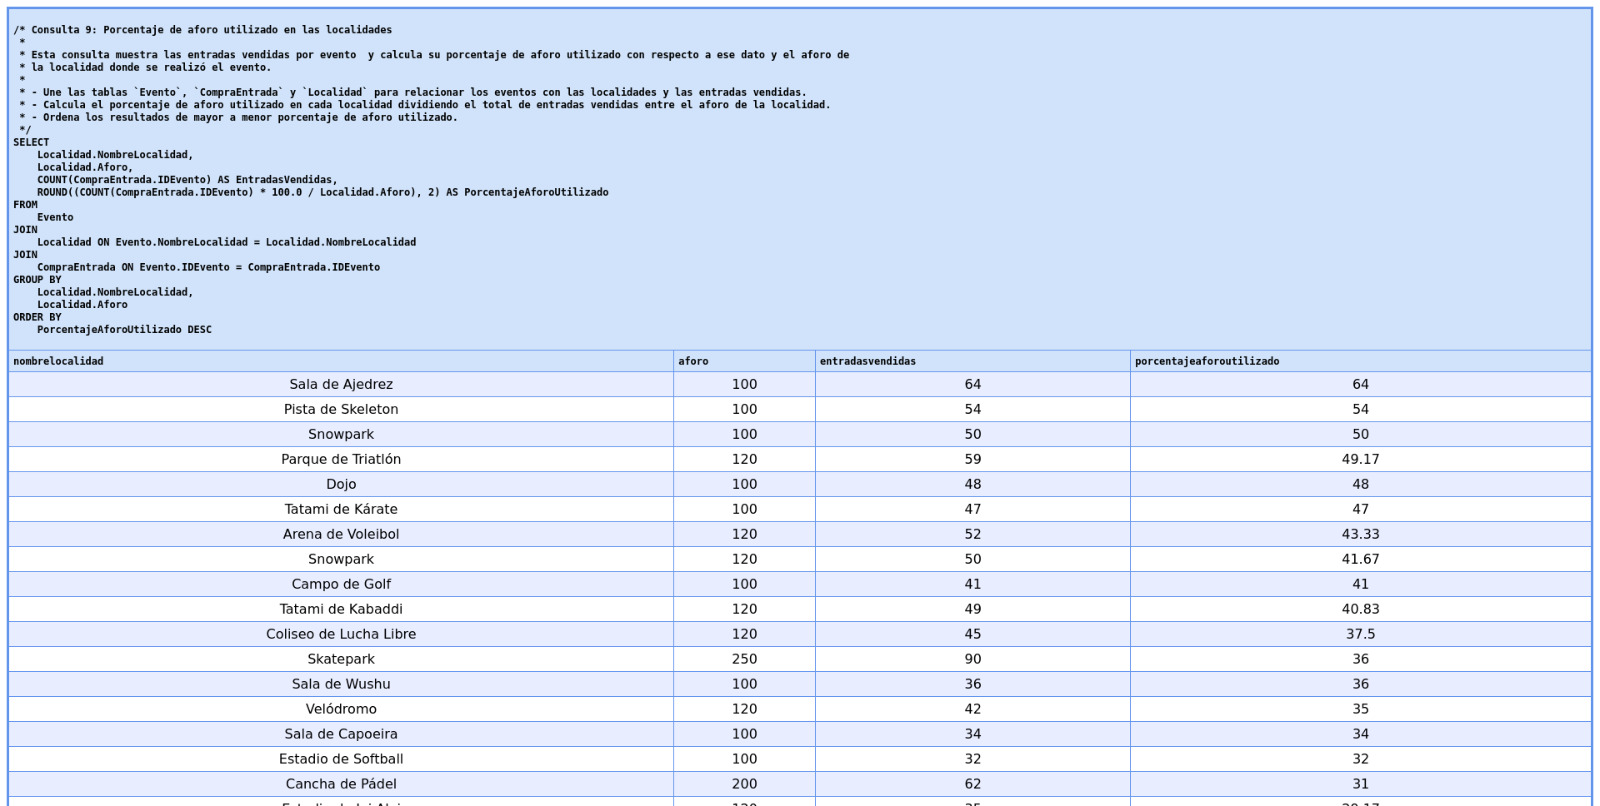
\includegraphics[width=16.5cm]{resources/Chapters/Consultas/Imagenes/Consulta9.jpg} 
	
	Consulta 9. Porcentaje de aforo utilizado en las localidades.
\end{center}

\textbf{Propósito de la consulta}

La consulta tiene como objetivo calcular el porcentaje de aforo utilizado en cada localidad para eventos realizados, considerando el número total de entradas vendidas y la capacidad máxima (aforo) de cada localidad. Además, se ordenan los resultados de mayor a menor porcentaje de aforo utilizado.

\textbf{Desglose de la consulta}

\begin{itemize} \item \textbf{Selección de columnas (\texttt{SELECT}):} \begin{itemize} \item \texttt{Localidad.NombreLocalidad}: Identifica el nombre de la localidad donde se realizó cada evento. \item \texttt{Localidad.Aforo}: Representa la capacidad máxima (número total de asientos) de cada localidad. \item \texttt{COUNT(CompraEntrada.IDEvento) AS EntradasVendidas}: Cuenta la cantidad total de entradas vendidas para eventos realizados en cada localidad. \item \texttt{ROUND((COUNT(CompraEntrada.IDEvento) * 100.0) / Localidad.Aforo, 2) AS PorcentajeAforoUtilizado}: Calcula el porcentaje de aforo utilizado en cada localidad, dividiendo las entradas vendidas entre el aforo y multiplicando por 100. La función \texttt{ROUND} redondea este valor a dos decimales. \end{itemize}
	
	\item \textbf{Tablas involucradas (\texttt{FROM} y \texttt{JOIN}):} \begin{itemize} \item \texttt{Evento}: Tabla que contiene información sobre los eventos realizados, incluyendo su relación con las localidades. \item \texttt{Localidad}: Tabla que almacena datos sobre las localidades, incluyendo su nombre y capacidad máxima (\texttt{Aforo}). \item \texttt{CompraEntrada}: Tabla que registra las entradas compradas para cada evento. \item \textbf{Unión de tablas (\texttt{JOIN})}: \begin{itemize} \item \texttt{Evento.NombreLocalidad = Localidad.NombreLocalidad}: Relaciona cada evento con la localidad donde se realizó. \item \texttt{Evento.IDEvento = CompraEntrada.IDEvento}: Conecta cada evento con las entradas vendidas correspondientes. \end{itemize} \end{itemize}
	
	\item \textbf{Agrupación de resultados (\texttt{GROUP BY}):} \begin{itemize} \item La agrupación se realiza por: \begin{itemize} \item \texttt{Localidad.NombreLocalidad}: Para obtener estadísticas específicas para cada localidad. \item \texttt{Localidad.Aforo}: Para incluir el aforo máximo en los cálculos por localidad. \end{itemize} \end{itemize}
	
	\item \textbf{Ordenamiento de resultados (\texttt{ORDER BY}):} \begin{itemize} \item Los resultados se ordenan por \texttt{PorcentajeAforoUtilizado} en orden descendente (\texttt{DESC}), destacando las localidades con mayor porcentaje de uso de su capacidad. \end{itemize} \end{itemize}

\textbf{Análisis detallado}

\begin{itemize} \item \textbf{Relación entre tablas:} \begin{itemize} \item Cada entrada registrada en \texttt{CompraEntrada} está asociada a un evento específico (\texttt{Evento}). \item Cada evento se realiza en una localidad particular (\texttt{Localidad}), estableciendo la conexión para calcular el porcentaje de entradas vendidas respecto al aforo de esa localidad. \end{itemize}
	
	\item \textbf{Uso de funciones agregadas:} \begin{itemize} \item \texttt{COUNT(CompraEntrada.IDEvento)}: Cuenta el total de entradas vendidas para eventos realizados en cada localidad. \item \texttt{ROUND}: Redondea el cálculo del porcentaje a dos decimales para mejorar la presentación de los datos. \end{itemize}
	
	\item \textbf{Cálculo del porcentaje de aforo utilizado:} \begin{itemize} \item La fórmula \texttt{(COUNT(CompraEntrada.IDEvento) * 100.0) / Localidad.Aforo} calcula la proporción de entradas vendidas respecto al aforo máximo y la convierte en un porcentaje. \end{itemize}
	
	\item \textbf{Ordenamiento por porcentaje:} \begin{itemize} \item Ordenar los resultados por \texttt{PorcentajeAforoUtilizado} permite identificar las localidades donde se aprovechó más la capacidad disponible. \end{itemize} \end{itemize}

\textbf{Posibles escenarios y consideraciones}

\begin{itemize} \item \textbf{Localidades sin entradas vendidas:} \begin{itemize} \item Si una localidad no tiene eventos con entradas vendidas, no aparecerá en los resultados debido al uso de \texttt{COUNT}, que excluye valores nulos. \end{itemize}
	
	\item \textbf{Capacidad máxima (aforo):} \begin{itemize} \item Localidades con un aforo bajo pueden tener un porcentaje de uso alto incluso con pocas entradas vendidas, lo que podría sesgar los análisis si no se consideran otros factores. \end{itemize}
	
	\item \textbf{Localidades con eventos múltiples:} \begin{itemize} \item Si una localidad ha albergado varios eventos, el porcentaje de aforo utilizado considera la suma total de entradas vendidas en todos los eventos realizados en esa localidad. \end{itemize} \end{itemize}

Esta consulta permite evaluar la eficiencia en el uso de las capacidades de las localidades, proporcionando información útil para optimizar la planificación de eventos futuros.